\documentclass{llncs}
\usepackage{amsmath,amssymb,amsfonts,stmaryrd}
\usepackage{graphicx}
\usepackage{color}
\usepackage{listings}
\lstset{
   basicstyle=\scriptsize\ttfamily,
   frame=single,
   breaklines=true,
}
\usepackage{hyperref}
\usepackage{tikz}
\usetikzlibrary{arrows}
\usepackage{algorithm}
\usepackage{algpseudocode}
\usepackage[T1]{fontenc}

%%%%%
\newcommand{\sylvain}[1]{\textcolor{red}{#1}}
\newcommand{\francois}[1]{\textcolor{blue}{#1}}
\newcommand{\david}[1]{\textcolor{green}{#1}}

\newcommand\for{\mathbin{\text{\it for}}}
\newcommand\inhibits{\mathbin{-\!\Yleft}}
\newcommand\activates{\rightarrow}
\newcommand{\I}[1]{\mathit{#1}}

\newcommand{\ra}{\rightarrow}
\newcommand{\lra}{\longrightarrow}

\DeclareMathOperator{\Set}{Set}

\begin{document}
\bibliographystyle{splncs03}


\title{Influence Systems vs Reaction Systems}

\author{Fran\c{c}ois Fages\inst{1} \and Thierry Martinez\inst{2} \and
   David A.\ Rosenblueth\inst{1,3} \and \mbox{Sylvain Soliman\inst{1}}}

\institute{Inria Saclay-\^Ile-de-France, Team Lifeware, France\\
   \email{Francois.Fages@inria.fr} \email{Sylvain.Soliman@inria.fr}
   \and
   Inria Paris, SED, France \email{Thierry.Martinez@inria.fr}
%   \and National Autonomous University of Mexico\\ \email{drosenbl@unam.mx}}
   \and Instituto de Investigaciones en Matem\'aticas Aplicadas y en Sistemas (IIMAS), Universidad Nacional Aut\'onoma de M\'exico (UNAM) \email{drosenbl@unam.mx}}

\maketitle



\begin{abstract}

   In Systems Biology, modelers develop more and more re\-action-based models to
   describe the mechanistic biochemical reactions underlying cell processes.
   They may also work, however, with a simpler formalism of influence graphs,
   to merely describe the positive and negative influences between molecular species.
   The first approach is promoted by reaction model exchange formats such as
   SBML, and tools like CellDesigner,
   while the second is supported by other tools that have been historically
   developed to reason about boolean gene regulatory networks.
   In practice, modelers often reason with both kinds of formalisms,
%   and may find it useful to use an influence model
   and may find an influence model useful
   in the process of building a reaction model.
   In this paper, we introduce a formalism of influence systems with forces,
   and put it in parallel with reaction systems with kinetics,
   in order to develop a similar hierarchy of boolean, discrete, stochastic and differential semantics.
   We show that the expressive power of influence systems is the same as
   that of reaction systems under the differential semantics,
   but weaker under the other interpretations, in the sense that some discrete
   behaviours of reaction systems cannot be expressed by influence systems.
   This approach leads us to consider a positive boolean semantics which we compare
   to the asynchronous semantics of gene regulatory networks \emph{\`a la} Thomas.
   We study the monotonicity properties of the positive boolean semantics
   and derive from them an efficient algorithm to compute attractors.
   %These concepts are illustrated with models from the literature.
\end{abstract}


\section{Introduction}

In Systems Biology, modelers develop more and more reaction models to describe the biochemical reactions underlying cell processes.
This approach is promoted by reaction-model exchange formats such as SBML~\cite{Hucka03bi}
and by the subsequent creation of large reaction-based model repositories such as BioModels~\cite{NBBCDDLSSSSH06nar},
without prejudging of their interpretation by differential equations, Markov chains, Petri nets, or boolean transition systems \cite{FS08tcs}.

Modelers can also work, however, with a simpler formalism of \emph{influence systems}
to merely describe the positive and negative influences between molecular species,
without fixing their implementation with biochemical reactions.
In particular, boolean influence systems have been popularized in the 70's by Glass, Kauffman \cite{GK73jtb}
and Thomas \cite{Thomas73jtb,TA90book}
to reason about gene regulatory networks, represented by ordinary graphs between genes
given with a boolean transition table which defines their synchronous or asynchronous boolean transition semantics.
Necessary conditions for multi-stability (cell differentiation) and oscillations (homeostasis) have been given in terms of
positive or negative circuits in the influence graph \cite{RRT08aam,Ruet16mfcs}.
Several tools such as GINsim~\cite{NBFLTC09bs}, GNA~\cite{BBCdJDGMMPRR12} or Griffin~\cite{RMCA14alcob},
use these properties and powerful graph-theoretic and model-checking techniques to automate reasoning
about the boolean state transition graph, compute attractors and verify various reachability and path properties.
The representation of boolean influence systems by Petri nets was described in~\cite{Chaouiya07bioinfo}
%but leads to quite complicated encodings.
but leads to complicated encodings.
It is also worth mentioning that influence systems with spatial information have been nicely developed in~\cite{Chazelle12cacm}
as a formalism particularly suitable for describing natural algorithms
in life sciences and social dynamics.

  In Systems Biology, modelers often reason with both kinds of formalisms, and may find it useful to use and maintain an influence model
  in the process of building a reaction model,
  for instance in order to reduce it
while preserving the essential influence circuits~\cite{NRTC09cmsb}.
One reason is that it is easier to visualize influence systems,
rather than reaction systems for which %quite
complicated graphical conventions such as SBGN~\cite{sbgn09nb}
have been developed.
  While it is clear that the influence graph is an abstraction of the reaction hypergraph~\cite{FS08tcs},
  and perhaps more surprisingly that the Jacobian influence system derived
  from the differential semantics of a reaction system is largely independent of the kinetics~\cite{FS08fmsb},
  influence models are mostly used for their graphical representation and their boolean semantics,
  but more rarely as a modeling paradigm for systems biology with quantitative semantics using differential equations, or stochastic semantics.
  
  In this paper, we introduce a formalism of influence systems with forces, which we put in parallel with reaction systems with kinetics,
  in order to develop a similar hierarchy of boolean, discrete, stochastic and differential semantics for influence systems,
  similarly to what is done for reasoning about programs in the framework of abstract interpretation~\cite{CC77popl,FS08tcs}.
  We show that the expressive power of influence systems is the same as that of reaction systems under the differential semantics,
  but is weaker under the other interpretations, in the sense that some formal discrete behaviours of reaction systems cannot be expressed
  by influence systems.
  This approach provides an influence model with a hierarchy of possible interpretations related by precise abstraction relationships,
  so that, for instance, if a behavior is not possible in the boolean semantics, it is surely not possible
  in the stochastic semantics whatever the influence forces are.
  
   This leads us to consider a positive boolean semantics which we compare
   to the asynchronous semantics of gene regulatory networks \emph{\`a la} Thomas.
   We study the monotonicity properties of the positive boolean semantics
   and derive from them an efficient algorithm to compute attractors.
These concepts are illustrated with models from the literature.
  
\section{Preliminaries on Reaction Systems with Kinetics}

%\subsection{Notations}

In this article, unless explicitly noted, we will denote by capital letters
(e.g. $S$) sets or multisets, by bold letters (e.g., $\vec x$) vectors and by
small roman or Greek letters elements of those sets or vectors (e.g.~real
numbers, functions).
For a multiset $M$, let $\Set(M)$ denote the set obtained from the support of
$M$, and brackets like $M(i)$ denote the multiplicity in the multiset (usually
the stoichiometry).
$\geq$ will denote the pointwise order for vectors, multisets and sets (i.e.
inclusion).

\subsection{Syntax}

We recall here definitions from~\cite{FGS15tcs,FS08fmsb} for directed reactions with inhibitors:

\begin{definition}
A \emph{reaction} over molecular species $S = \{x_1,\dots,x_s\}$
is a quadruple $(R,M,P,f)$, also noted $f \for R / M \Rightarrow P$,
where $R$ is a multiset of \emph{reactants}, $M$ a set of \emph{inhibitors},
$P$ a multiset of \emph{products}, all composed of elements of $S$,
and $f:\mathbb{R}^s\rightarrow\mathbb{R}$, called \emph{kinetic expression},
is a mathematical function over molecular species concentrations.
A \emph{reaction system} is a finite set of reactions.
\end{definition}

It is worth noting that a molecular species in a reaction can be both a reactant and a product (i.e. a catalyst),
or both a reactant and an inhibitor (e.g. Botts--Morales enzymes \cite{Katsumata72jtb}).
Such molecular species are not distinguished in SBML and both are called reaction \emph{modifiers}.
Unlike SBML, we find it useful to consider only directed reactions (reversible reactions being represented here by two reactions)
and to enforce the following compatibility conditions between the kinetic expression and the structure of a reaction.

\begin{definition}[\cite{FGS15tcs,FS08fmsb}]\label{defi:rwell}
A reaction $(R,M,P,f)$ 
over molecular species $\{x_1,\dots,x_s\}$
is \emph{well formed} if the following conditions hold:
\begin{enumerate}
\item $f(x_1,\dots,x_s)$ is a partially differentiable function, non-negative
   on $\mathbb{R}_+^s$;
\item $x_i\in R$ if and only if ${\partial {f}}/ {\partial x_i}(\vec x)>0$ for some value $\vec x\in\mathbb{R}_+^s$;
\item $x_i\in M$ if and only if ${\partial {f}}/ {\partial x_i}(\vec x)<0$ for some value $\vec x\in\mathbb{R}_+^s$.
\end{enumerate}
A reaction system is well formed
if all its reactions are well formed.
\end{definition}


\begin{example}\label{LV}
  The classical prey-predator model of Lotka--Volterra can be represented by the following well-formed reaction system
  (without reaction inhibitors) between a proliferating prey $A$ and a predator $B$:
   \begin{lstlisting}
k1*A*B for A+B=>2*B.
k2*A for A=>2*A.
k3*B for B=>_.
   \end{lstlisting}
\end{example}



\subsection{Hierarchy of Semantics}

As detailed in~\cite{FS08tcs}, a reaction system can be interpreted with different formalisms
that are formally related by abstraction relationships in the framework of abstract interpretation \cite{CC77popl}
and form a hierarchy of semantics.
We simply recall here the definitions of the different semantics of a reaction system.

The \emph{differential} semantics corresponds to the association of
      an Ordinary Differential Equation (ODE) system with the reactions in the
      usual way:
      \[\frac{dx_j}{dt} = \sum_{(R_i, M_i, P_i, f_i)}(P_i(j) - R_i(j))\times f_i\]
      It is worth noting that in this interpretation, the inhibitors are supposed to decrease the reaction rate but do not prevent the reaction from
      proceeding with effects on the products and reactants.
      For instance, in Ex.~\ref{exLV}, we get the classical Lotka--Volterra equations $dB/dt = k1*A*B-k3*B$, $dA/dt = k2*A-k1*A*B$,
and the well-known oscillations between the concentrations of the prey and the predator.

The \emph{stochastic semantics} for reaction systems defines
transitions between discrete states describing numbers of each molecule, i.e.~vectors $\vec x$ of $\mathbb{N}^s$.
A transition is enabled if there are enough reactants,
and the reaction propensity is defined by the kinetics:
      $$\forall (R_i, M_i, P_i, f_i), {\vec x}\lra_S^{f_i}{\vec x'} \text{ with propensity}f_i\text{ if } {\vec x}\geq R_i, {\vec x'} = {\vec x} - R_i + P_i$$
Transition probabilities between discrete states are obtained through
normalization of the propensities of all enabled reactions,
and the time of next reaction can be computed
from the rates \emph{\`a la} Gillespie~\cite{Gillespie77jpc}.
      In this interpretation, the inhibitors are supposed to decrease the reaction propensity but do not prevent the reaction from occurring.
      They are thus ignored here by the stochastic transition conditions as in the differential semantics.
      In Ex.~\ref{LV}, the stochastic interpretation can exhibit some oscillations similar to the differential interpretation,
      and (almost surely) the extinction of the predator.

      The \emph{discrete}, or \emph{Petri Net}, semantics is similar but ignores the kinetics
      and is thus a trivial abstraction of the stochastic semantics by a forgetful functor:
      $$\forall (R_i, M_i, P_i, f_i), {\vec x}\lra_D{\vec x'}\text{ if }      {\vec x}\geq R_i, {\vec x'} = {\vec x} - R_i + P_i$$

The \emph{boolean semantics} is similar to the \emph{discrete} one
but on boolean vectors $x$ of $\mathbb{B}^s$,
obtained by the ``zero, non-zero'' abstraction of integers.
With this abstraction, when the number of a molecule is decremented,
it can still remain present, or become absent. It is thus necessary to take into account all the possible
complete consumption or not of the reactants in order to obtain a correct boolean abstraction
of the discrete and stochastic semantics \cite{FS08tcs}. The \emph{boolean transition system} $\lra_B$ is thus defined by:\\

\noindent
$\forall (R_i, M_i, P_i, f_i), \forall C\in{\cal P}(\Set(R_i)), {\vec       x}\lra_B{\vec x'}$
if ${\vec x}\supseteq \Set(R_i), {\vec x'} =       {\vec x} \setminus C \cup \Set(P_i)$

It is worth remarking that in Ex.~\ref{exLV} under this boolean interpretation, one can observe either
the stable coexistence of the prey and the predator, or the extinction of the predator with or without the preceding extinction of the prey.

As proven in~\cite{FS08tcs}, the last three of these semantics are
related by successive Galois connections, which means that \emph{if a behaviour is not possible in the boolean semantics,
it is not possible in the stochastic semantics} whatever the reaction kinetics are.
On the other hand, the first differential semantics is not an abstraction but
rather a limit of the first one for high number of molecules, as shown for instance
in~\cite{Gillespie77jpc}.

It is worth noticing that the set of inhibitors of a reaction is just a syntactical annotation
which has not been used to define the different semantics of the hierarchy.
One can also consider a \emph{boolean semantics with negation}
where the set of inhibitors of a reaction is seen as a conjunction of negative conditions for the transition
(disjunctions can be represented with several reactions). The \emph{boolean with negation transition system} $\lra_{BN}$ is then defined by:

$\forall (R_i, M_i, P_i, f_i) \forall C\in{\cal P}(\Set(R_i)) {\vec       x}\lra_{BN}{\vec x'}$

\hfill if ${\vec x}\supseteq \Set(R_i), {\vec x}\cap M_i=\emptyset, {\vec x'} =       {\vec x} \setminus C \cup \Set(P_i)$\\
However, this strict interpretation of inhibitors by negations restricts the set of possible boolean transitions
and is not compatible with the differential semantics, since in that interpretation an inhibitor may just slightly decrease the rate of a reaction without preventing it from proceeding.


\subsection{Influence Graph of a Reaction System}

Here we recall two definitions of the influence graph associated with a reaction
system, and their equivalence under general assumptions~\cite{FS08fmsb,FGS15tcs}.
The first definition is based on the Jacobian matrix $J$ formed of the partial derivatives 
$J_{ij} = {\partial \dot{x_i}}/ {\partial x_j}$, where $\dot{x_i}$ is defined by the differential semantics.

\begin{definition}\label{DIG}

The \emph{differential influence graph} associated with a reaction system is the
graph having for vertices the molecular species, and for edge-set the
following two kinds of edges:

\begin{tabular}{r}
   $\{A\ra^+B\ |\ {{\partial \dot{x_B}}/ {\partial x_A}} >0$ for some value $\vec x\in\mathbb{R}_+^s\}$\\
   $\cup\{A\ra^-B\ |\ {{\partial \dot{x_B}}/{\partial x_A}} <0$ for some value $\vec x\in\mathbb{R}_+^s\}$
\end{tabular}

\end{definition}

\begin{definition}

The \emph{syntactical influence graph} associated with a reaction system $M$ is
the graph having for vertices the molecular species, and for edges the
following set of positive and negative influences:

\begin{tabular}{lll}
&$\{A\ra^+B\ |$&$\exists (R_i, M_i, P_i, f_i)\in M$, $(R_i(A)>0$ and $P_i(B)-R_i(B)>0)$\\
&& or $(A\in M_i$ and $P_i(B)-R_i(B)<0)\}$\\
&$\cup\{A\ra^-B\ |$&$\exists (R_i, M_i, P_i, f_i)\in M$, $(R_i(A)>0$ and $P_i(B)-R_i(B)<0)$ \\
&&or $(A\in M_i$ and $P_i(B)-R_i(B)>0)\}$\\
\end{tabular}

\end{definition}

The syntactical graph is trivial to
compute, in linear time, by browsing the syntax of the rules.
Both definitions are equivalent under general assumptions:


\begin{theorem}[\cite{FGS15tcs,FS08fmsb}]
For any well-formed reaction system
such that the syntactical influence graph contains no conflict (i.e.~no pair of the form $A\ra^+ B$ and $A\ra^- B$),
the syntactical and differential influence graphs are identical.
  \end{theorem}




\section{Influence Systems with Forces}

Reaction systems allow the description of mechanistic models of cell processes, but
modelers can also work with a simpler formalism of \emph{influence systems}
to merely describe the positive and negative influences between molecular species,
without fixing their implementation with biochemical reactions.
In this section, we propose a syntax for influence systems with forces which allows us to define
a hierarchy of differential, stochastic, discrete and positive boolean semantics, similarly to reaction systems.
We then focus on different boolean semantics, and compare them to Thomas's setting for gene regulatory networks.


\subsection{Syntax}

The idea is to syntactically distinguish conjunctive from disjunctive conditions by writing influences with several sources for representing a conjunction of conditions,
while the different influences on a same target express a disjunction of conditions.
These syntactical conventions are %similar to the formalism of process hitting \cite{PH} and
a particular case of the concept of multiplexes introduced in \cite{BCK08esm} restricted here to disjunctive normal forms.

\begin{definition}

   Given $S = \{x_1,\dots,x_s\}$ a set of species, an \emph{influence system}
   $I$ is a set of quintuples $(P, N, t, \sigma, f)$ called \emph{influences},
   where $P\subset S$ is called the \emph{positive sources} of the influence, $N\subset S$ the \emph{negative sources}, $t\in S$ is the \emph{target}, 
   \emph{sign} $\sigma\in\{+,-\}$ is the sign of the influence, and $f$ is a real-valued mathematical function
   of $\mathbb{R}^s$, called the \emph{force} of the influence.

\end{definition}

Influences of sign $+$ will be called \emph{positive influences} and those of
sign $-$, \emph{negative influences}.
In addition, we distinguish the positive sources from the negative sources in an influence (positive or negative),
in order to annotate the fact that in the differential semantics,
the source increases or decreases the force of the influence,
and in the boolean semantics with negation whether the source or the negation of the source
is a condition for a change in the target.

For practical reasons we provide an ASCII syntax for influence systems which is used in Biocham\footnote{\url{http://lifeware.inria.fr/biocham}} v4: they
will be written as sequences of lines, where each set is written as a
comma-separated sequence of the corresponding species, where the sign is
represented as an arrow separating sources from the target, \lstinline|->| for positive influences,
and \lstinline+-<+ for negative influences, and where the positive and negative sources are separated
by a \lstinline|/| that can be omitted if there is no negative source.

Let us now define the concept of \emph{well-formed} influence
systems similarly to the above Def.~\ref{defi:rwell} for reaction systems,
with a particular condition for the target of a negative influence, as follows:

\begin{definition}
   An influence $(P, N, t, \sigma, f)$
over molecular species $\{x_1,\dots,x_s\}$
is \emph{well formed} if the following conditions hold:
\begin{enumerate}
\item $f(x_1,\dots,x_s)$ is a partially differentiable function, non-negative
   on $\mathbb{R}_+^s$;
\item $x_i\in P$ if and only if $\sigma = +$ (resp.\ $-$) and
   ${\partial {f}}/ {\partial x_i}(\vec x)>0$ (resp.\ $<0$) for some value
   $\vec x\in\mathbb{R}_+^s$;
\item $x_i\in N$ if and only if $\sigma = +$ (resp.\ $-$) and
   ${\partial {f}}/ {\partial x_i}(\vec x)<0$ (resp.\ $>0$) for some value
  $\vec x\in\mathbb{R}_+^s$;
  \item $t\in P$ if $\sigma=-$.
\end{enumerate}
An influence system is well formed if all its influences are
well formed.
\end{definition}

\begin{example}\label{exLV}
   The prey-predator model of Lotka--Volterra of Ex.~\ref{LV} can also be represented by the following well-formed influence system %between the prey $A$ and the predator $B$:
   \begin{lstlisting}
k1*A*B for A,B -< A.
k1*A*B for A,B -> B.
k2*A for A -> A.
k3*B for B -< B.
   \end{lstlisting}
   composed of four influences with positive sources only,
   $(\{A, B\}, \emptyset, A, -, k1*A*B)$, $(\{A, B\}, \emptyset, B, +, k1*A*B)$, $(\{A\}, \emptyset, A, +, k2*A)$ and $(\{B\}, \emptyset, B, -, k3*B)$.

\end{example}


\subsection{Hierarchy of Semantics}

Given a set of species $S=
\{x_1,\dots,x_s\}$ and an influence system $I$ over $S$, 
the \emph{differential} semantics associates the following ODE system with $I$:

\[
   \frac{dx_k}{dt} = \sum_{(P_i, N_i, x_k, +, f_i) \in I}f_i - \sum_{(P_j, N_j, x_k, -, f_j) \in I}f_j
\]
Intuitively, it adds up all the forces of the positive influences on $x_k$ and
subtracts all forces of negative influences on $x_k$ in the derivative of
$x_k$ over time.
For instance, in Ex.~\ref{exLV}, we get the same equations as for Ex.~\ref{LV}. 

It is worth noticing that the negative sources in a well-formed influence
decrease the force of the influence but do not disable it.
Consequently, we define similarly the \emph{stochastic} semantics of an influence system with forces,
by a transition system, noted $\lra_S$, between discrete states, i.e.~vectors $\vec x$ of $\mathbb{N}^s$,
with the condition that the positive sources are present in sufficient number,
with a transition propensity defined by the force,
and the target updated as follows:
      $$\forall (P_i, N_i, A_i, \sigma_i, f_i), {\vec x}\lra_S^{f_i}{\vec x'} \text{ with propensity}f_i\text{ if } {\vec x}\geq P_i, {\vec x'} = {\vec x}\  \sigma_i\ A_i$$
Transition probabilities between discrete states are obtained through
normalization of the propensities of all enabled transitions,
and the time of next reaction can also be given \emph{\`a la} Gillespie~\cite{Gillespie77jpc}.
      In this interpretation, the negative sources are supposed to decrease the influence propensity but do not prevent the influence from proceeding.
      They are thus ignored here by the stochastic transition conditions.

      The \emph{discrete} (or \emph{Petri Net}) semantics simply ignores the forces:
      $$\forall (P_i, N_i, A_i, \sigma_i, f_i), {\vec x}\lra_D{\vec x'}\text{ if }      {\vec x}\geq P_i, {\vec x'} = {\vec x}\ \sigma_i\ A_i$$

The \emph{positive boolean semantics} is defined on boolean vectors $x$ of $\mathbb{B}^s$,
by the ``zero, non-zero'' abstraction of integers of the discrete semantics. Unlike reaction systems, this boolean semantics associates one transition with one influence:
$$\forall (P_i, N_i, A_i, \sigma_i, f_i), {\vec       x}\lra_B{\vec x'}\text{
if }{\vec x}\geq P_i, {\vec x'} =       {\vec x}\ \sigma_i\ A_i$$
This boolean semantics is positive in the sense that it ignores the negative sources of an influence
and contains no negation in the influence enabling condition.
In Ex.~\ref{exLV} we get the same boolean transitions as in Ex.~\ref{LV}, although in general one can expect to get more transitions (as shown below in Sec.~\ref{express}).


With these definitions, one can obtain as in \cite{FS08tcs}, a hierarchy of semantics related by simple abstraction relationships (Galois connections in the framework of abstract interpretation \cite{CC77popl})
which allows us to state, for instance, that if a behaviour is not possible in the positive boolean semantics, it is also not possible in the discrete or stochastic semantics for any forces.


\subsection{Influence Graph of an Influence System}

One can define the differential influence graph of an influence system
as in Def.~\ref{DIG} for reaction systems, and get a similar equivalence result with the following

\begin{definition}

The \emph{syntactical influence graph} associated with an influence system $M$ is
the graph having for vertices the molecular species, and for edges the
following set of positive and negative influences:

\begin{tabular}{lll}
&$\{A\ra^+B\ |$&$\exists (P_i, N_i, B, \sigma_i, f_i)\in M$, $(A\in P_i$ and $\sigma_i=+)$\\
&& or $(A\in N_i$ and $\sigma_i=-)\}$\\
&$\cup\{A\ra^-B\ |$&$\exists (P_i, N_i, B, \sigma_i, f_i)\in M$, $(A\in P_i$ and $\sigma_i=-)$ \\
&&or $(A\in N_i$ and $\sigma_i=+)\}$\\
\end{tabular}

\end{definition}

\begin{proposition}
For a well-formed influence system
such that the syntactical influence graph contains no conflict,
the syntactical and differential influence graphs are identical.
  \end{proposition}
\begin{proof}

   Recall that $\dot{x_B} = \sum_{(P_i, N_i, x_B, +, f_i) \in I}f_i -
   \sum_{(P_j, N_j, x_B, -, f_j) \in I}f_j$

   Hence $\frac{\partial \dot{x_B}}{\partial x_A} = \sum_{(P_i, N_i,
   x_B, +, f_i) \in I}\frac{\partial f_i}{\partial x_A} - \sum_{(P_j, N_j,
   x_B, -, f_j) \in I}\frac{\partial f_j}{\partial x_A}$

   Since the SIG does not have any conflict, $A\ra^+B$ is in the SIG (a
   similar reasoning can be made for $A\ra^-B$) \emph{iff}

   $%\[
      \frac{\partial \dot{x_B}}{\partial x_A} = \sum_{(P_i, N_i, x_B, +, f_i)
      \in I, A\in P_i, A\not\in N_i}\frac{\partial f_i}{\partial x_A} - \sum_{(P_j,
      N_j, x_B, -, f_j) \in I, A\not\in P_j, A\in N_j}\frac{\partial f_j}{\partial x_A}
   $%\]

   Now, since the influence system is well formed, all terms of the left-hand
   sum are non-negative ($A\not\in N_i$) and strictly positive for some points
   $\vec x_i$ and all terms of the right-hand sum are non-positive ($A\not\in
   P_j$) and strictly negative for some $\vec x_j$.

   We have that $A\ra^+B$ in the SIG \emph{iff} the above sum has at least one
   term, which is equivalent to the existence of some $\vec x$ in the state
   space where one of the terms above is non-null, and therefore
   $\frac{\partial \dot{x_B}}{\partial x_A} >0$, i.e., $A\ra^+B$ is in the
   DIG.\qed

\end{proof}

\subsection{Expressive Power Compared to Reaction Systems}\label{express}

\begin{theorem}\label{reprInflu}

  Any (well-formed) influence system with forces can be represented by a (well-formed) reaction system with kinetics,
  with the same boolean, discrete, stochastic and differential semantics.

\end{theorem}
\begin{proof}
  Let us represent a positive influence $f \for P/N \rightarrow t$ 
  by a catalytic synthesis reaction $f \for P/N\Rightarrow P+t$.

  Similarly, let us represent a negative influence $f \for P/N \inhibits t$,
  by an active degradation reaction $f \for P+t/N\Rightarrow P$.

  It is straightforward to verify that the boolean, discrete, stochastic as well as differential
  semantics recalled and defined above are the same.

  Furthermore, the well-formedness condition is preserved.
  Indeed, this property only depends on the
  forces/kinetic expressions and on the reactants/inhibitors, which %and those 
  do not change through that transformation thanks to the condition that in
  \emph{well-formed} influence systems. In addition, $t \in P$ in the case of the
  negative influence.
  \qed

\end{proof}

This theorem shows that an influence system can be simulated by a reaction system for the different semantics.
The converse does not hold for the boolean semantics, for instance.
Indeed, let us consider boolean semantics of the reaction $C\Rightarrow A+B$ (the kinetics is omitted).
  We have a transition from the state $(A,B,C)=(0,0,1)$ to $(1,1,0)$ which is obviously
  not possible in an influence system since only one variable can change in one transition.  
However, the converse holds for the differential semantics:

\begin{theorem}
Under the differential semantics, (well-formed) influence and reaction systems have the same expressive power.
\end{theorem}
\begin{proof}

   For each reaction $(R, M, P, f)$ of a given
   reaction system, let us add the following influences:

   \begin{gather*}
      (\Set(R), \Set(M), x_i, +, (P(i) - R(i))\times f) \text{ when } P(i) - R(i) > 0\\
      (\Set(R), \Set(M), x_i, -, (R(i) - P(i))\times f) \text{ when } P(i) - R(i) < 0
   \end{gather*}

      The associated ODE system collects all $(P_i - R_i)\times
   f$ exactly as in the differential semantics of the original reaction
   system. Furthermore, it is easy to check that these influences are well formed since the
   original reaction is well formed and the force is only a positive integer
   multiplied by the original kinetic expression. 
\qed
\end{proof}

This theorem shows that as far as the differential semantics is concerned,
the influence systems have the same expressive power as reaction systems
and there is no theoretical reason to develop a reaction model.
This does not mean that there is a canonical reaction system associated with an influence system.
Generally, different implementations with reactions are possible without changing the differential semantics.
They represent extra information that is irrelevant to the analysis or simulation of the differential equations,
but could lead to different stochastic simulations, for instance.


\subsection{Boolean Semantics with Negation}

One can also consider a boolean semantics with negation for influence systems,
where the negative sources are interpreted as negations in the enabling condition.
Formally, the \emph{boolean with negation semantics} of an influence system is then defined by the following transition system:
$$\forall (P_i, N_i, A_i, \sigma_i, f_i), {\vec       x}\lra_B{\vec x'}\text{
if }{\vec x}\geq P_i,\ {\vec x}\cap N_i=\emptyset,\ {\vec x'} =       {\vec x}\ \sigma_i\ A_i$$

This interpretation allows us to represent more boolean transition semantics.
Let us call a \emph{unitary transition system}, a transition system that updates \emph{at most one} variable of $\vec x$ in each transition.
It is worth remarking that in this case, the state transition graph lives on a hypercube (e.g.~Fig.~\ref{fig:bernot_influences} of Sec.~\ref{ex}).



\begin{proposition}\label{propUnitary}
  Any unitary boolean transition system can be represented
  by an influence system under the boolean semantics with negation.
\end{proposition}
\begin{proof}
It is sufficient to notice that since a unitary boolean transition 
$s \longrightarrow_{\I{BN}} s'$ changes at most one species, say $x_i$, from $s$ to $s'$,
it can be represented by either a positive influence, $(P,N,x_i,+)$, if $s'(x_i)=1$,
or a negative influence, $(P,N,x_i,-)$, if $s'(x_i)=0$,
with $P=\{x \mid s(x)=1\}$ and $N=\{x \mid s(x)=0\}$.
\qed
\end{proof}


Let us call a \emph{positive boolean transition system} one that contains no negation in the conditions for enabling a transition,
i.e.~if a transition is enabled when $s(x_i)=0$ then it is also enabled when $s(x_i)=1$.

\begin{corollary}
  Any unitary positive boolean transition system can be represented
  by an influence system under the positive boolean semantics.
\end{corollary}
\begin{proof}
  In the influence system associated by Prop.~\ref{propUnitary} with a positive unitary transition system,
  any influence that has negative sources is doubled by a counterpart influence where such sources are positive (by definition of positive boolean transition system).
  Therefore, in the associated influence system, the negative sources can be simply ignored, as done by the positive boolean semantics.
  \qed
  \end{proof}


\subsection{Functional Boolean Semantics with Negation \emph{\`a la} Thomas}
  

The boolean semantics defined by Ren\'e Thomas originally for gene networks \cite{TA90book}, is \emph{functional}, in the sense that
the next boolean state ${\vec x}'$ is defined by a boolean function $\phi(\vec x)$, not a relation.
In this setting, the synchronous semantics is deterministic, and the non-deterministic asynchronous semantics
is obtained by interleaving, by considering all the possible transitions that change the boolean value of \emph{exactly one} of the genes at a time.
A truly non-deterministic influence system such as $\{(A,\emptyset,B,+,f),\ (A,\emptyset, B,-,g)\}$, for which the transition relation is not a function,
cannot be represented. 
Thomas's setting excludes self-loops in the state transition graph and all steady states are stable (i.e.~terminal states):


\begin{proposition}
  The boolean transition systems definable by Thomas's regulatory networks are the unitary boolean transition systems without self-loops.
\end{proposition}
\begin{proof}
  A Thomas's transition graph is necessarily unitary and without self-loops since each transition changes the boolean value of exactly (not at most) one variable at a time.
The converse follows from Prop.~\ref{propUnitary} by excluding the possibility of having self-loop transitions which change no variable.
  \qed
\end{proof}

This restriction to transition functions is even more striking in Thomas's multilevel setting, where the above
system can (in the discrete semantics) have transitions from $(1,1)$ both to
$(1,0)$ and to $(1,2)$. That would necessitate the corresponding logical
parameter for $B$ to be at the same time $<1$ and $>1$.
It is worth noting that despite this restriction, the logical formalism of Thomas is successfully used in a wide variety of models \cite{TFFT16bi,GCBRKT13plos,NCCT10pcb,GCT08bi} in systems biology.



\section{Properties of the Positive Boolean Semantics}

In this section, we focus on the positive boolean semantics of influence systems and study its
properties. 
Recall that $\leq$ denotes the
pointwise order on $\{0,1\}$ coordinates of vectors representing states.

\begin{proposition}[Monotonicity]
   \label{prop:mono}
   The positive boolean semantics of influence systems is monotonic: let $I$ be an
   influence system over $S=\{x_1,\dots,x_s\}$ and $v_1, v_2$ be two boolean
   states, i.e., vectors of $\mathbb{B}^s$

   \noindent
   \begin{minipage}[c]{0.8\textwidth}
      \[\text{if } v_1\leq v_2\text{ then }\forall v'_1, v_1\lra
      v'_1,\exists v'_2, v'_1\leq v'_2 \text{ and } v_2\lra v'_2\]
   \end{minipage}%
   \begin{minipage}[c]{0.2\textwidth}
      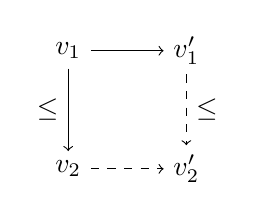
\begin{tikzpicture}
         [node distance=15mm]
         \node (v1) {$v_1$};
         \node (v2) [below of=v1] {$v_2$};
         \node (vp1) [right of=v1] {$v'_1$};
         \node (vp2) [right of=v2] {$v'_2$};

         \draw[->] (v1) -- (vp1);
         \draw[->] (v1) -- node [left] {$\leq$} (v2);
         \draw[->,dashed] (v2) -- (vp2);
         \draw[->,dashed] (vp1) -- node [right] {$\leq$} (vp2);
      \end{tikzpicture}
   \end{minipage}

\end{proposition}

\begin{proof}

   One can simply notice that since there are no
   negations in the enabling conditions, any influence that is enabled in $v_1$ is also
   enabled in $v_2$.\qed

\end{proof}

It is worth noticing that this monotonicity property for transitions is fundamentally different from that of
monotone dynamical systems~\cite{AS03tac} which are deterministic, and therefore impose the monotonicity property on
the \emph{unique} image of $v_1$ and $v_2$.
In our setting, Prop.~\ref{prop:mono} states that there exists some $v'_2\geq v'_1$, but
the existence of negative influences in the system permits that some other images of $v_2$ might not
be greater than $v'_1$. Nevertheless, we have

\begin{proposition}[Greatest element]
   \label{prop:greatest}
   Let $C$ be a Terminal Strongly Connected Component (TSCC) of the state transition
   graph of a positive influence system, then $C$ has a greatest element:
$\exists v_0\in C, \forall v\in C, v\leq v_0$

\end{proposition}

\begin{proof}

   Let us prove this proposition by contradiction: assume that there are two
   incomparable maximal elements $v_1$ and $v_2$ in $C$. Since $C$ is strongly
   connected there is a path from $v_1$ to $v_2$ and along that path a state
   $v_3$ and its successor in the path $v_4$ such that $v_3\leq v_1$ and
   $v_4\not\leq v_1$, as $v_2\not\leq v_1$. Now, using Prop.~\ref{prop:mono}
   we get that $v_1\lra v'_1$ with $v_4\leq v'_1$ and $v'_1\in C$ since
   $C$ is terminal. However $v'_1$ is either greater or less than $v_1$ since
   it is the result of applying a single influence. If $v_1 < v'_1$ we have
   a contradiction as we supposed $v_1$ maximal. If $v'_1\leq v_1$ we get
   $v_4\leq v_1$ by transitivity and that is also contradictory. \qed

\end{proof}

\begin{corollary}

   To enumerate the attractors, i.e., TSCCs, of a positive influence system,
   it is enough to check the strongly connected components (SCCs) of states
   that have no strictly increasing transition.

\end{corollary}

\begin{proof}

   This is an immediate consequence of Prop.~\ref{prop:greatest} as each TSCC
   can be represented by its greatest element which has no strictly
   increasing transition. \qed

\end{proof}

Notice that stable states are a particular case with no strictly decreasing
transition either.
Moreover, any strictly decreasing transition should be
``reversible'' for the SCC to be a TSCC. This allows us to rule out potential
TSCC candidates without exploring their whole SCC in Alg.~\ref{alg:tscc}
(implementation available in Biocham v4).

\begin{algorithm}[htb]
\begin{algorithmic}
   \Procedure{list\_tscc\_candidates}{}
   \State $Constraints\gets\{P\wedge\neg N\implies t\mid (P, N, +, t, f)\in
      I\}$\\
   \Comment{Enabled positive influences must not change the state}
   \State $Candidates\gets$\Call{EnumerateSolutions}{$Constraints$}
   \For{$C\in Candidates$}
      \If{$C$ has no strictly decreasing transition}
      \State $C$ is a \emph{stable} steady state
      \ElsIf{$C$ has a non-reversible strictly decreasing transition}
      \State $C$ is \emph{not} in a TSCC
      \Else
      \State $C$'s SCC must be explored to check if it is a TSCC
      \EndIf
   \EndFor
   \EndProcedure
   \Function{EnumerateSolutions}{$Constraints$}
      \State Iteratively solve by SAT/CP the CSP defined by $Constraints$
      \State \Return The set of solutions
   \EndFunction
\end{algorithmic}
\caption{TSCC maximal elements candidates enumeration algorithm} 
\label{alg:tscc}
\end{algorithm}

\begin{proposition}

   Given an influence system, there is at least one TSCC of the original
   influence system in each TSCC of its positive semantics.

\end{proposition}
\begin{proof}

   The positive semantics only adds transitions by enabling more influences,
   it can therefore only merge TSCCs. \qed

\end{proof}

This result suggests finding complex attractors of non-positive systems,
such as logical models \emph{\`a la} Thomas \cite{RRT08aam,Ruet16mfcs}, by enumerating
the greatest elements of the TSCCs of their positive boolean semantics, and then looking for
attractors of the original system.
This approach provides an over-approximation of the attractors
and is complementary to recent works which provide lower-bounds on their
number~\cite{KBS14acri}.

\section{Examples}\label{ex}

\subsection{Influence Model of p53/Mdm2 DNA Damage Repair System~\cite{AOK09jtb}}

The p53/Mdm2 DNA damage repair system is an interesting oscillatory system which has been first modeled in \cite{CCT07plos}
by a reaction system with differential equations, and then in \cite{AOK09jtb} and \cite{OAK10jtb} by simplified influence systems with discrete and differential semantics respectively.

We illustrate here the search for TSCCs with two versions of the influence model of \cite{AOK09jtb}.
In the first model, we simply
   transcribe  the graph of Fig.~4 of the
   authors as a boolean influence system. We therefore ignore the multi-level aspect they developed.
In the second model, we add some activations on p53 and DNA-damage, and an inhibition on
   cytoplasmic Mdm2, in order to take into account some basal state of the
   model.
   The influence systems and the computed TSCCs are listed in the Biocham session depicted in Fig.~\ref{p53}.
      

\begin{figure}[htb]
\begin{center}
   \begin{minipage}[r]{.45\textwidth}
      \begin{center}
         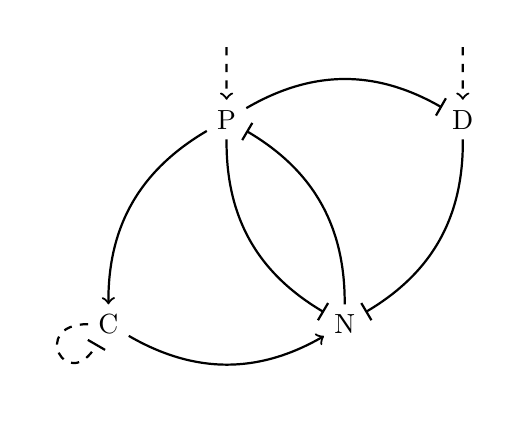
\begin{tikzpicture}[scale=1.5, thick]
            \node (C) at (0, 0) {C};
            \node (N) at (2, 0) {N};
            \node (P) at (1, 1.732) {P};
            \node (toP) at (1, 2.432) {};
            \node (D) at (3, 1.732) {D};
            \node (toD) at (3, 2.432) {};

            \draw[->] (P) to[bend right] (C);
            \draw[->] (C) to[bend right] (N);
            \draw[-|] (P) to[bend right] (N);
            \draw[-|] (N) to[bend right] (P);
            \draw[-|] (P) to[bend left] (D);
            \draw[-|] (D) to[bend left] (N);

            \draw[dashed,-|] (C) to[out=180, in=240, looseness=7] (C);
            \draw[dashed,->] (toP) -- (P);
            \draw[dashed,->] (toD) -- (D);
         \end{tikzpicture}
      \end{center}
   \end{minipage}
   \begin{minipage}[c]{.3\textwidth}
   \end{minipage}
   \begin{minipage}[l]{.5\textwidth}
      \lstinputlisting{kaufman.log}
   \end{minipage}\hfill
\end{center}
\caption{{Left:} Influence graph displayed in Fig.~4 of~\cite{AOK09jtb}, without the
      activation multi-levels.
      The dashed influences are those added in our second version of the
      model.
{Right:} Biocham v4 session for computing the TSCC in both influence systems.} \label{p53}
\end{figure}


   Our algorithm shows that there is in each case a single complex attractor (i.e.~not marked as stable or not terminal),
   accordingly to \cite{AOK09jtb}, and four
   stable steady states in the first case.
   Note that in \cite{OAK10jtb}, this influence model was further extended with differential and stochastic dynamics
   which could be represented in our setting by influence forces.

\subsection{Influence Model of the Mammalian Circadian Clock~\cite{CBDDMC12pcs}}

A good example of the use of logical models \emph{\`a la} Thomas is the recent
paper by Comet et al.~\cite{CBDDMC12pcs} studying different variants of small models of the
circadian rhythms in mammals.
A direct import in Biocham v4 of the logical model of Section~5 of~\cite{CBDDMC12pcs} gives
the following influence system with negative sources:
\lstinputlisting{bernot.bc}

The positive semantics of this system is %actually quite
close to the original boolean semantics with negation \emph{\`a la Thomas} of the model. They both have a single TSCC: the vector $(1, 1, 1)$ that is found by 
the command \verb|list_tscc_candidates| 
as sole candidate.
Furthermore, only
a few state transitions become reversible in the positive boolean semantics, while they are
irreversible in the original boolean semantics with negation \emph{\`a la Thomas} of the model, as depicted in Fig.~\ref{fig:bernot_influences}.

\begin{figure}[htb]
\begin{center}
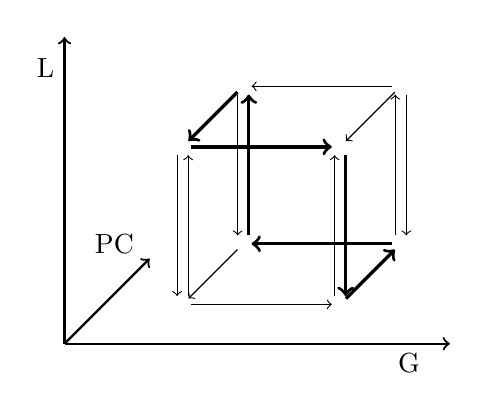
\begin{tikzpicture}
   [->,shorten >=3pt,shorten <=3pt]
   \begin{scope}[shorten <=0pt,thick,very near end]
      \draw (-1.5, -0.5, 0) -- node [below] {G} (3.5, -0.5, 0);
      \draw (-1.5, -0.5, 0) -- node [left] {L} (-1.5, 3.5, 0);
      \draw (-1.5, -0.5, 0) -- node [above left] {PC} (-1.5, -0.5, -3);
   \end{scope}

   \draw (0, 0, 0) -- (2, 0, 0);
   \draw[very thick] (2, 0, 0) -- (2, 0, -2);
   \draw[very thick] (2, 0, -2) -- (0, 0, -2);
   \draw (0, 0, -2) -- (0, 0, 0);
   \draw (2, 2, -2) -- (0, 2, -2);
   \draw[very thick] (0, 2, -2) -- (0, 2, 0);
   \draw[very thick] (0, 2, 0) -- (2, 2, 0);
   \draw (2, 2, -2) -- (2, 2, 0);

   \draw[xshift=-2pt] (2, 0, 0) -- (2, 2, 0);
   \draw[very thick,xshift=2pt] (2, 2, 0) -- (2, 0, 0);
   \draw[xshift=-2pt] (0, 2, -2) -- (0, 0, -2);
   \draw[very thick,xshift=2pt] (0, 0, -2) -- (0, 2, -2);
   \draw[xshift=-2pt] (0, 2, 0) -- (0, 0, 0);
   \draw[xshift=2pt] (0, 0, 0) -- (0, 2, 0);
   \draw[xshift=-2pt] (2, 0, -2) -- (2, 2, -2);
   \draw[xshift=2pt] (2, 2, -2) -- (2, 0, -2);
\end{tikzpicture}
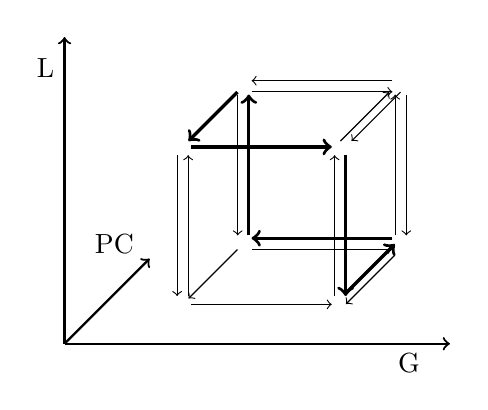
\begin{tikzpicture}
   [->,shorten >=3pt,shorten <=3pt]
   \begin{scope}[shorten <=0pt,thick,very near end]
      \draw (-1.5, -0.5, 0) -- node [below] {G} (3.5, -0.5, 0);
      \draw (-1.5, -0.5, 0) -- node [left] {L} (-1.5, 3.5, 0);
      \draw (-1.5, -0.5, 0) -- node [above left] {PC} (-1.5, -0.5, -3);
   \end{scope}

   \draw (0, 0, 0) -- (2, 0, 0);
   \draw[very thick,yshift=2pt] (2, 0, 0) -- (2, 0, -2);
   \draw[yshift=-2pt] (2, 0, -2) -- (2, 0, 0);
   \draw[very thick,yshift=2pt] (2, 0, -2) -- (0, 0, -2);
   \draw[yshift=-2pt] (0, 0, -2) -- (2, 0, -2);
   \draw (0, 0, -2) -- (0, 0, 0);
   \draw[yshift=2pt] (2, 2, -2) -- (0, 2, -2);
   \draw[yshift=-2pt] (0, 2, -2) -- (2, 2, -2);
   \draw[very thick] (0, 2, -2) -- (0, 2, 0);
   \draw[very thick] (0, 2, 0) -- (2, 2, 0);
   \draw[xshift=2pt] (2, 2, -2) -- (2, 2, 0);
   \draw[xshift=-2pt] (2, 2, 0) -- (2, 2, -2);

   \draw[xshift=-2pt] (2, 0, 0) -- (2, 2, 0);
   \draw[very thick,xshift=2pt] (2, 2, 0) -- (2, 0, 0);
   \draw[xshift=-2pt] (0, 2, -2) -- (0, 0, -2);
   \draw[very thick,xshift=2pt] (0, 0, -2) -- (0, 2, -2);
   \draw[xshift=-2pt] (0, 2, 0) -- (0, 0, 0);
   \draw[xshift=2pt] (0, 0, 0) -- (0, 2, 0);
   \draw[xshift=-2pt] (2, 0, -2) -- (2, 2, -2);
   \draw[xshift=2pt] (2, 2, -2) -- (2, 0, -2);
\end{tikzpicture}
\end{center}
\caption{State transition graphs of the model under, \textbf{Left:} the boolean semantics with negation \emph{\`a la} Thomas, similar to Fig.~7
of~\cite{CBDDMC12pcs}, \textbf{Right:} the positive boolean semantics, where
some state transitions have become reversible.}
\label{fig:bernot_influences}
\end{figure}

The approximation introduced by the positive boolean semantics can be explained by quantitative dynamics considerations.
For instance, when $G$ is on, the transcription leading to the
PER-CRY complexes is stimulated, however~\cite{CBDDMC12pcs} explains that
these complexes can only migrate to the nucleus in absence of light. This
\emph{absence} cannot be checked in a positive semantics model, however the
consensus mechanistic process is rather thought to be a modulation of PER
transcription by light (see for instance~\cite{LG03pnas} for the mammalian
case). Being purely quantitative, it is not easy to take into account such a
regulation in a boolean model except with the reversible activation of $PC$
when $G$ is on, whether $L$ is on or not. This is what happens in our positive
model as can be seen in the right panel of Fig.~\ref{fig:bernot_influences},
and it is similar to what happens for the light in the original model.

The same reasoning explains the reversible inactivation of $G$ when $PC$ is
active. Indeed there is a basal synthesis of $G$ that cannot check, in a
positive setting, that $PC$ is inactive in order to activate the genes. Once
again, the mechanistic process is a quantitative inhibition of the CLOCK-BMAL1
complexes by PER-CRY and a conservative boolean approximation of that process
is reflected by the reversible activation of $G$ in presence of $PC$.

In \cite{CBDDMC12pcs}, the authors also restrict the possible behaviours by introducing delays
for the boolean transitions which could be considered as a further expansion of the formalism.




\section{Discussion}

In this paper, we hope to have clarified some differences between influence systems and reaction systems,
and especially some subtle discrepancies between the precise boolean semantics that have been considered in the literature.
As far as the modeling of one biological system is concerned, the modeler can work with one formalism and one tool
to answer the questions about their model. Nevertheless, as soon as different modeling tools are to be used,
or the model has to be communicated and reused for another purpose, understanding and mastering these discrepancies in the semantics
of the interactions becomes crucial.

We have shown that, for influence systems and reaction systems with inhibitors, one can obtain
a hierarchy of semantics %related by formal abstractions (Galois connections)
which goes from the concrete stochastic semantics to a discrete Petri net, and then a positive boolean semantics
in which the inhibitors of the reactions or influences are just ignored.
This is consistent with the fact that the inhibitors decrease the rate or force
in the quantitative semantics, but do not really prevent the reaction or influence from proceeding.
This convention thus ensures that all discrete behaviours are approximated when we go up in the abstractions of the hierarchy of semantics,
and that if a behaviour is not possible in the positive boolean semantics (which can be checked by model-checking methods for instance)
it is not possible in the stochastic semantics for any forces.
Furthermore, we have shown that in the positive boolean semantics, the monotonicity of the
transition relation allows us to enumerate the complex attractors more efficiently by restricting the search to the greatest elements candidates.

On the other hand, the boolean semantics \emph{\`a la} Thomas of influence systems,
interprets inhibitors as negations, and %excludes self-loops (on non-terminal states).
contains a restriction on the definition of the transition relation by a function, not a relation, which limits the sources of non-determinism.
We have shown that the boolean semantics with negation leads to a more expressive formalism
in which any unitary boolean transition system can be encoded,
but does not correspond to an abstraction of the stochastic semantics,
unless the stochastic transitions interprets inhibitors as negative conditions
which does not correspond to the differential semantics.
With the functional restriction, we have proven that each TSCC in the positive semantics
contains at least one TSCC of the semantics \emph{\`a la} Thomas,
and thus that our algorithm can be used to prune the search space in this setting also.

We have also shown that reaction systems and influence systems
have the same expressive power under the differential semantics.
This means that, as far as the differential equations are concerned,
the details given in the reactant-product structure of a reaction system
are not necessary, and that the same differential equations can be derived
from an influence system with forces.
Several reaction systems can be associated with an influence system
with the same differential semantics.
This leaves open the design of canonical forms for reaction systems, and computer tools for automatically maintaining
the implementation of an influence system
by a reaction system.



\subsubsection*{Acknowledgements.}
We are grateful to Paul Ruet for interesting discussions on Thomas's framework, and to the reviewers for their comments.
This work was partially supported by ANR project Hyclock under contract
ANR-14-CE09-0011, and PASPA-DGAPA-UNAM, Conacyt grants 221341 and 261225.


\bibliography{contraintes}

\appendix

\end{document}

OLD STUFF


In the boolean semantics of an influence system, 
one reasons about the presence and absence of the molecular species only,
and the forces of the influences are ignored.
A \emph{boolean state} $s$ is a boolean function of the species $S\mapsto\mathbb{B}$. It
will often be written equivalently as the set of species with image 1. These
species are \emph{present} (or \emph{expressed}) in the state.
Those with image 0 are \emph{absent}.

One can consider a boolean semantics in which inhibitors are seen as negative conditions for enabling a transition, as follows:

\begin{definition}
   An influence $(P, N, t, \sigma)$ is \emph{enabled} in boolean state $s$ when
   $\forall p\in P, s(p) = 1$ and $\forall n\in N, s(n) = 0$.

\end{definition}

Following this definition, the different sources of an influence represent a conjunction of positive and negative conditions.
Note that an influence $(P, N, t, +)$ such that $P \cap N \not= \emptyset$ is not enabled for any state,
and that a positive (resp.\ negative) influence with its target in the positive (resp.\ negative) sources does not change the state.
This motivates the following:


\begin{definition}

   A \emph{proper influence} is an influence $(P, N, t, +)$ (resp.\ $(P, N, t, -)$) such that
   $t \in N$ (resp.\ $t \in P$).
   The \emph{proper version of an influence} $(P, N, t, +)$ (resp.\ $(P, N, t, -)$) is $(P, N\cup\{t\}, t, +)$ (resp.\ $(P\cup\{t\}, N, t, -)$).
   
\end{definition}

\begin{definition}
\label{BN}
  The boolean semantics with negation of an influence system $I$ is given by the transition relation $\longrightarrow_{\I{BN}}:(S\mapsto\mathbb{B})\mapsto(S\mapsto\mathbb{B})$
   such that $s \longrightarrow_{\I{BN}} s'$ 
   if influence $(P, N, t, +)$ (resp.\ $(P, N, t, -)$) is  enabled
   in $s$ and
   \[
      s'(x) = \begin{cases}
         1 \text{(resp.\ $0$)} & \text{if $x = t$},\\
         s(x) & \text{otherwise}
      \end{cases}
   \]
   or if there is no influence enabled in $s$, and $s'=s$.

\end{definition}

Unlike \cite{CRMT03posta}, states with no influence enabled are completed here by a self-loop to avoid deadlocks, so as to define a right-total transition relation (i.e.~a Kripke structure),
as required by temporal logic specifications of behaviors and model-checking tools \cite{CGP99mit}.
This is a common convention for the modeling of gene regulatory networks~\cite{JGHPSG04bmb} and in tools like GINsim~\cite{NBFLTC09bs}, GNA~\cite{BBCdJDGMMPRR12} or Griffin~\cite{RMCA14alcob}
for instance.

By considering the disjunctive normal form (DNF) of logical formulae,
one can show that under the boolean semantics with negation, influence systems can represent any \emph{unitary} transition system, i.e.~asynchronuous transition system that updates at most one variable in each transition.


\begin{proposition}\label{propUnitary}
  Any unitary boolean transition system can be represented
  by an influence system under the boolean semantics with negation.
\end{proposition}
\begin{proof}
Note that in a transition $s \longrightarrow_{\I{BN}} s'$ at most one species changes image from $s$ to $s'$.
Self-loops are taken care of by not having any enabled influence in states with a self-loop. % the last case of Definition~\ref{BN}.
Hence, we need only have influences for the cases when one species changes image.
If a species $t$ changes image from $0$ (resp.\ $1$) to $1$ (resp.\ $0$), then the corresponding influence system has the influence $(P,N,t,+)$ (resp.\ $(P,N,t,-)$) such that $\forall p\in P, s(p) = 1$ and $\forall n\in N, s(n) = 0$.
It is easy to see that  $(P,N,t,+)$ (resp.\ $(P,N,t,-)$) will be enabled exactly when $t$ changes image from $0$ (resp.\ $1$) to $1$ (resp.\ $0$) in $s \longrightarrow_{\I{BN}} s'$.
\end{proof}


